\section{A brief introduction to LP and MIP}

In this section we provide a very brief introduction to linear programming and mixed integer programming.
The goal is simply to introduce the necessary vocabulary in order to simplify the wording of the remaining
of this chapter.

A linear programming is a central tool in optimization that allows one to solve mathematical models whose objective
is a linear function and whose constraints are representable by linear inequalities. A linear function is a function
$f : \mathbb{R}^n \rightarrow \mathbb{R}$ such that
$$
f(x_1, \ldots, x_n) = c_1 x_1 + \dots + c_n x_n 
$$
for some constants $c_1, \ldots, c_n \in \mathbb{R}$. A linear inequality is an inequality of the form
$$
a_1 x_1 + \ldots + a_n x_n \geq b
$$
for $a_1, \ldots, a_n, b \in \mathbb{R}$. In general, we have not one but $m$ constraints so we are given an $m \times n$ matrix of 
coefficients $A$ and $m$ values $b_1, \ldots, b_m$. Each row of coefficients represents one constant. The general form of a linear program is the following:

\begin{center}
\begin{tabular}{rcccccccccc}
$\displaystyle \mathbf{min}$ & $c_1 x_1$ & $+$ & $c_2 x_2$ & $+$ & $\ldots$ & $+$ & $c_n x_n$ & & \\
\textbf{s.t} & $a_{11} x_1$ & $+$ & $a_{12} x_2$ & $+$ & $\ldots$ & $+$ & $a_{1n} x_n$ & $\geq$ & $b_1$ \\
             & $a_{21} x_1$ & $+$ & $a_{22} x_2$ & $+$ & $\ldots$ & $+$ & $a_{2n} x_n$ & $\geq$ & $b_2$ \\
             & $\vdots$ & & & & & & & & $\vdots$ \\
             & $a_{m1} x_1$ & $+$ & $a_{m2} x_2$ & $+$ & $\ldots$ & $+$ & $a_{mn} x_n$ & $\geq$ & $b_m$ \\[0.2cm]
& $x_i \in \mathbb{R}$ & & & & & & & &
\end{tabular}
\end{center}

Numerous problems can be modeled as linear programs. This, combined with the fact that linear programs can be solved efficiently,
makes LP a very interesting problem solving tool \cite{lp1, lp2}.

Every linear program is associated with another linear program called its \emph{dual} LP. The original problem is called the \emph{primal}.
The dual of a LP has one constraint for each variable of the primal and one variable for each constraint of the primal. The objective function
is reversed so that if the primal is a minimization problem then the dual is a maximization problem (and vice-versa). The main result
about LP duality is the \emph{strong duality theorem} \cite{lp3} which states that the primal has an optimal solution if and only if the dual also has one 
and both of them have the same value. The dual of a LP can be obtained by following a systematic procedure. In the case of the LP formulated above,
the dual is given by:

\begin{center}
\begin{tabular}{rcccccccccc}
$\displaystyle \mathbf{max}$ & $b_1 y_1$ & $+$ & $b_2 y_2$ & $+$ & $\ldots$ & $+$ & $b_m y_m$ & & \\
\textbf{s.t} & $a_{11} y_1$ & $+$ & $a_{21} y_2$ & $+$ & $\ldots$ & $+$ & $a_{m1} y_m$ & $\leq$ & $c_1$ \\
             & $a_{12} y_1$ & $+$ & $a_{22} y_2$ & $+$ & $\ldots$ & $+$ & $a_{m2} y_m$ & $\leq$ & $c_2$ \\
             & $\vdots$ & & & & & & & & $\vdots$ \\
             & $a_{1n} x_1$ & $+$ & $a_{2n} y_2$ & $+$ & $\ldots$ & $+$ & $a_{mn} y_m$ & $\leq$ & $c_n$ \\[0.2cm]
& $y_i \in \mathbb{R}$ & & & & & & & &
\end{tabular}
\end{center}

We are going to exploit duality when developing our CG solution. In our algorithm we will denote a function \textsf{LP-solve} that,
given an LP, outputs its optimal solution $x$, the optimal solution of the dual $y$ and the optimal objective value.

In the above formulation we assumed that the domain of the variables was $\mathbb{R}$. Linear programs remain easy to solve as long as the
variable ranges are continuous ranges. A lot of very important problems can be modeled with a linear objective function and
linear constraints but require integral variable domains. We refer to these problems as integer programs (IP) or mixed integer program (MIP)
if some of the variables are continuous and some are integral. The duality theory mentioned above does not extend to integer programming.
The general integer programming problem is \NPhard. 
This makes it much more challenging to find optimal solutions to MIP's in general. In this chapter's introduction we mentioned that
Problem \ref{prob:tep} was hard to solve but Problem \ref{prob:tep-mul} was easy. We will see that both problems can be formulated with nearly the same
model. The only difference between them is that the first requires integer variables whereas the second allows for continuous variables.

A lot of research has been put towards finding efficient algorithms for solving MIP's \cite{wolsey}. For the algorithms developed here,
we denote a function  \textsf{MIP-solve} that given a MIP (or IP), outputs the optimal solution $x$ and the optimal objective value.

%Even tought are all linear program, throughout this thesis we use the convention that whenver we refer to a model as a LP then we are assuming that 
%all variables have defined over continuous range.

To give a concrete example of a linear program, we model Problem \ref{prob:tep-mul}. A classic way to formulate Problem 
\ref{prob:tep-mul} as a linear program is to express it as a Multi-commodity flow (MCF) problem \cite{steven}.
We define variables $x_{ed}$ for each edge $e \in E(G)$ and demand $d \in \mathcal{D}$ such that the value of $x_{ed}$ represents the faction
of $\vol(d)$ that traverses edge $e$. The model LP is the following:

\begin{center}
\begin{tabular}{crcllr}
\multicolumn{5}{l}{$\mcflp(G, \mathcal{D})$} \\[0.5cm] 
$\displaystyle \mathbf{min}$ & $\lambda$ & & & & \\[0.5cm]
$\textbf{s.t.}$ & $\displaystyle \sum_{d \in \mathcal{D}} x_{ed} \cdot \vol(d)$                               & $\leq$ & $\lambda \cdot \bnd(e)$ & $\forall e \in E(G)$ & (1) \\[0.5cm]
                & $\displaystyle \sum_{e \in \delta^-(v)} x_{ed} - \sum_{e \in \delta^+(v)} x_{ed}$ & $=$    & $ 0$ & $\forall v \in V(G) \setminus \{ s_i, t_i \},$  & (2) \\[-0.2cm]
                &  &  &  & $\forall d \in \mathcal{D}$ \\[0.5cm]
                & $\displaystyle \sum_{e \in \delta^-(s)} x_{ed} - \sum_{e \in \delta^+(s)} x_{ed}$ & $=$    & $-1$ & $\forall i \in \{ 1, \ldots, r \},$ & (3) \\[-0.2cm]
                &  &  &  & $\forall d = (s, t, \nu) \in \mathcal{D}$ \\[0.5cm]
                & $\displaystyle \sum_{e \in \delta^-(t)} x_{ed} - \sum_{e \in \delta^+(t)} x_{ed}$ & $=$    &  $1$ & $\forall i \in \{ 1, \ldots, r \},$ & (4) \\[-0.2cm] 
                &  &  &  & $\forall d = (s, t, \nu) \in \mathcal{D}$ \\[0.5cm]
                & $x_{ed}$ & $\in$ & $[0, 1]$ \\[0.5cm]
                & $\lambda$ & $\geq$ & $0$
\end{tabular}
\end{center}

Constraints (1) ensure that the total demand volume traversing any edge is at most a fraction $\lambda$ of its capacity. Constraints (2), (3) and (4) are known
as \emph{flow constraints} and ensure that each demand $d$ is routed from $\src(d)$ to $\dst(d)$. More precisely, the group of constraints (3) makes sure that the whole
demand exits $\src(d)$ and the group of constraints (4) ensure that the whole demand reaches $\dst(d)$. The constraints (2) ensure that no demand traffic is lost by
requiring that any fraction of the demand that enters an intermediate router also exits it.

Given a solution matrix $x$ to \mcflp~we can easily construct a set of paths for each demand $d = (s, t, \nu) \in \mathcal{D}$.
To do so, we perform a sequence of breadth-first searches (BFS) from $s$ following only edges $e$ such that $x_{ed} > 0$. Each time we reach $t$, we 
trace back the path $p$ and reduce the value of $x_{ed}$ by the $\min_{e \in E(p)} x_{ed}$. We continue to do this until one of the searches
fails to reach $t$. At this point we finished computing a set of paths for demand $d$. Repeating the process for each demand will yield a set of 
paths over which we can route the demands without exceeding the capacity of any edge by a factor greater than $\lambda$. 

Figure \ref{fig:flow-path} illustrates this process on a small example. The graph represents the values of $x_{ed}$ for a specific demand $d$. Each edge
if labeled with the value of $x_{ed}$ (for clarity, we ommit edges with value $0$ since they are ignored anyway by the DFS). Then the blue arrows show possible
BFS paths. After each path is found, the value of the edges is reduced until no more path exists. In this case we get three paths: 
$((\node{a}, \node{b}), (\node{b}, \node{d}))$, $((\node{a}, \node{c}), (\node{c}, \node{d}))$ and $((\node{a}, \node{b}), (\node{b}, \node{c}), (\node{c}, \node{d}))$.

\begin{figure}
\begin{center}
\begin{tabular}{c c c}
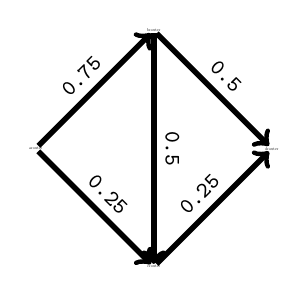
\begin{tikzpicture}
\node[scale=0.15] (a) at (0, 0) {\router{a}{router}};
\node[scale=0.15] (b) at (1.5, 1.5) {\router{b}{router}};
\node[scale=0.15] (c) at (1.5, -1.5) {\router{c}{router}};
\node[scale=0.15] (d) at (3, 0) {\router{d}{router}};
\draw[line width=2] (a) edge[above, sloped, ->] node[black,font=\bfseries] {\footnotesize \texttt{0.75}} (b);
%\draw[line width=2] (b) edge[below, sloped, bend left = 10, ->] node[black,font=\bfseries] {\tiny \texttt{0}} (a);

\draw[line width=2] (a) edge[above, sloped, ->] node[black,font=\bfseries] {\footnotesize \texttt{0.25}} (c);
%\draw[line width=2] (c) edge[below, sloped, bend left = 10, ->] node[black,font=\bfseries] {\tiny \texttt{0}} (a);

\draw[line width=2] (b) edge[above, sloped, ->] node[black,font=\bfseries] {\footnotesize \texttt{0.5}} (d);
%\draw[line width=2] (d) edge[below, sloped, bend left = 10, ->] node[black,font=\bfseries] {\tiny \texttt{0}} (b);

\draw[line width=2] (c) edge[above, sloped, ->] node[black,font=\bfseries] {\footnotesize \texttt{0.25}} (d);
%\draw[line width=2] (d) edge[below, sloped, bend left = 10, ->] node[black,font=\bfseries] {\tiny \texttt{0}} (c);

\draw[line width=2] (b) edge[above, sloped, ->] node[black,font=\bfseries] {\footnotesize \texttt{0.5}} (c);
%\draw[line width=2] (c) edge[below, sloped, bend left = 10, ->] node[black,font=\bfseries] {\tiny \texttt{0}} (b);
\end{tikzpicture}

&

\begin{tikzpicture}
\node[scale=0.15] (a) at (0, 0) {\router{a}{router}};
\node[scale=0.15] (b) at (1.5, 1.5) {\router{b}{router}};
\node[scale=0.15] (c) at (1.5, -1.5) {\router{c}{router}};
\node[scale=0.15] (d) at (3, 0) {\router{d}{router}};
\draw[line width=2] (a) edge[above, sloped, ->] node[black,font=\bfseries] {\footnotesize \texttt{0.75}} (b);
%\draw[line width=2] (b) edge[below, sloped, bend left = 10, ->] node[black,font=\bfseries] {\tiny \texttt{0}} (a);

\draw[line width=2] (a) edge[above, sloped, ->] node[black,font=\bfseries] {\footnotesize \texttt{0.25}} (c);
%\draw[line width=2] (c) edge[below, sloped, bend left = 10, ->] node[black,font=\bfseries] {\tiny \texttt{0}} (a);

\draw[line width=2] (b) edge[above, sloped, ->] node[black,font=\bfseries] {\footnotesize \texttt{0.5}} (d);
%\draw[line width=2] (d) edge[below, sloped, bend left = 10, ->] node[black,font=\bfseries] {\tiny \texttt{0}} (b);

\draw[line width=2] (c) edge[above, sloped, ->] node[black,font=\bfseries] {\footnotesize \texttt{0.25}} (d);
%\draw[line width=2] (d) edge[below, sloped, bend left = 10, ->] node[black,font=\bfseries] {\tiny \texttt{0}} (c);

\draw[line width=2] (b) edge[above, sloped, ->] node[black,font=\bfseries] {\footnotesize \texttt{0.5}} (c);
%\draw[line width=2] (c) edge[below, sloped, bend left = 10, ->] node[black,font=\bfseries] {\tiny \texttt{0}} (b);


\draw[cyan, line width=2, ->] plot [smooth] coordinates { ($(a)+(0,0.5)$) ($(b)+(0,0.75)$) ($(d)+(0,0.5)$) };

\end{tikzpicture}

&

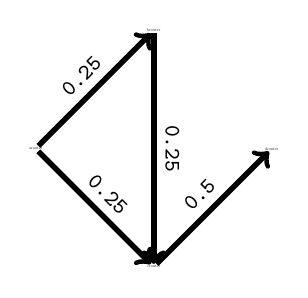
\begin{tikzpicture}
\node[scale=0.15] (a) at (0, 0) {\router{a}{router}};
\node[scale=0.15] (b) at (1.5, 1.5) {\router{b}{router}};
\node[scale=0.15] (c) at (1.5, -1.5) {\router{c}{router}};
\node[scale=0.15] (d) at (3, 0) {\router{d}{router}};
\draw[line width=2] (a) edge[above, sloped, ->] node[black,font=\bfseries] {\footnotesize \texttt{0.25}} (b);
%\draw[line width=2] (b) edge[below, sloped, bend left = 10, ->] node[black,font=\bfseries] {\tiny \texttt{0}} (a);

\draw[line width=2] (a) edge[above, sloped, ->] node[black,font=\bfseries] {\footnotesize \texttt{0.25}} (c);
%\draw[line width=2] (c) edge[below, sloped, bend left = 10, ->] node[black,font=\bfseries] {\tiny \texttt{0}} (a);

%\draw[line width=2] (b) edge[above, sloped, ->] node[black,font=\bfseries] {\footnotesize \texttt{1}} (d);
%\draw[line width=2] (d) edge[below, sloped, bend left = 10, ->] node[black,font=\bfseries] {\tiny \texttt{0}} (b);

\draw[line width=2] (c) edge[above, sloped, ->] node[black,font=\bfseries] {\footnotesize \texttt{0.5}} (d);
%\draw[line width=2] (d) edge[below, sloped, bend left = 10, ->] node[black,font=\bfseries] {\tiny \texttt{0}} (c);

\draw[line width=2] (b) edge[above, sloped, ->] node[black,font=\bfseries] {\footnotesize \texttt{0.25}} (c);
%\draw[line width=2] (c) edge[below, sloped, bend left = 10, ->] node[black,font=\bfseries] {\tiny \texttt{0}} (b);

\end{tikzpicture}

\\

(1) Solution graph

&

(2) First BFS

&

(3) Graph after reweight

\\[0.5cm]

\begin{tikzpicture}
\node[scale=0.15] (a) at (0, 0) {\router{a}{router}};
\node[scale=0.15] (b) at (1.5, 1.5) {\router{b}{router}};
\node[scale=0.15] (c) at (1.5, -1.5) {\router{c}{router}};
\node[scale=0.15] (d) at (3, 0) {\router{d}{router}};
\draw[line width=2] (a) edge[above, sloped, ->] node[black,font=\bfseries] {\footnotesize \texttt{0.25}} (b);
%\draw[line width=2] (b) edge[below, sloped, bend left = 10, ->] node[black,font=\bfseries] {\tiny \texttt{0}} (a);

\draw[line width=2] (a) edge[above, sloped, ->] node[black,font=\bfseries] {\footnotesize \texttt{0.25}} (c);
%\draw[line width=2] (c) edge[below, sloped, bend left = 10, ->] node[black,font=\bfseries] {\tiny \texttt{0}} (a);

%\draw[line width=2] (b) edge[above, sloped, ->] node[black,font=\bfseries] {\footnotesize \texttt{1}} (d);
%\draw[line width=2] (d) edge[below, sloped, bend left = 10, ->] node[black,font=\bfseries] {\tiny \texttt{0}} (b);

\draw[line width=2] (c) edge[above, sloped, ->] node[black,font=\bfseries] {\footnotesize \texttt{0.5}} (d);
%\draw[line width=2] (d) edge[below, sloped, bend left = 10, ->] node[black,font=\bfseries] {\tiny \texttt{0}} (c);

\draw[line width=2] (b) edge[above, sloped, ->] node[black,font=\bfseries] {\footnotesize \texttt{0.25}} (c);
%\draw[line width=2] (c) edge[below, sloped, bend left = 10, ->] node[black,font=\bfseries] {\tiny \texttt{0}} (b);

\draw[cyan, line width=2, ->] plot [smooth] coordinates { ($(a)+(0,-0.5)$) ($(c)+(0,-0.75)$) ($(d)+(0,-0.5)$) };


\end{tikzpicture}

&

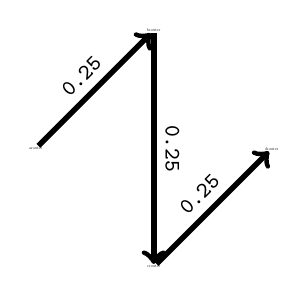
\begin{tikzpicture}
\node[scale=0.15] (a) at (0, 0) {\router{a}{router}};
\node[scale=0.15] (b) at (1.5, 1.5) {\router{b}{router}};
\node[scale=0.15] (c) at (1.5, -1.5) {\router{c}{router}};
\node[scale=0.15] (d) at (3, 0) {\router{d}{router}};
\draw[line width=2] (a) edge[above, sloped, ->] node[black,font=\bfseries] {\footnotesize \texttt{0.25}} (b);
%\draw[line width=2] (b) edge[below, sloped, bend left = 10, ->] node[black,font=\bfseries] {\tiny \texttt{0}} (a);

%\draw[line width=2] (a) edge[above, sloped, ->] node[black,font=\bfseries] {\footnotesize \texttt{1}} (c);
%\draw[line width=2] (c) edge[below, sloped, bend left = 10, ->] node[black,font=\bfseries] {\tiny \texttt{0}} (a);

%\draw[line width=2] (b) edge[above, sloped, ->] node[black,font=\bfseries] {\footnotesize \texttt{1}} (d);
%\draw[line width=2] (d) edge[below, sloped, bend left = 10, ->] node[black,font=\bfseries] {\tiny \texttt{0}} (b);

\draw[line width=2] (c) edge[above, sloped, ->] node[black,font=\bfseries] {\footnotesize \texttt{0.25}} (d);
%\draw[line width=2] (d) edge[below, sloped, bend left = 10, ->] node[black,font=\bfseries] {\tiny \texttt{0}} (c);

\draw[line width=2] (b) edge[above, sloped, ->] node[black,font=\bfseries] {\footnotesize \texttt{0.25}} (c);
%\draw[line width=2] (c) edge[below, sloped, bend left = 10, ->] node[black,font=\bfseries] {\tiny \texttt{0}} (b);

%\draw[cyan, line width=2, ->] plot [smooth] coordinates { ($(a)+(0,-0.5)$) ($(c)+(0,-0.75)$) ($(d)+(0,-0.5)$) };


\end{tikzpicture}

&

\begin{tikzpicture}
\node[scale=0.15] (a) at (0, 0) {\router{a}{router}};
\node[scale=0.15] (b) at (1.5, 1.5) {\router{b}{router}};
\node[scale=0.15] (c) at (1.5, -1.5) {\router{c}{router}};
\node[scale=0.15] (d) at (3, 0) {\router{d}{router}};
\draw[line width=2] (a) edge[above, sloped, ->] node[black,font=\bfseries] {\footnotesize \texttt{0.25}} (b);
%\draw[line width=2] (b) edge[below, sloped, bend left = 10, ->] node[black,font=\bfseries] {\tiny \texttt{0}} (a);

%\draw[line width=2] (a) edge[above, sloped, ->] node[black,font=\bfseries] {\footnotesize \texttt{1}} (c);
%\draw[line width=2] (c) edge[below, sloped, bend left = 10, ->] node[black,font=\bfseries] {\tiny \texttt{0}} (a);

%\draw[line width=2] (b) edge[above, sloped, ->] node[black,font=\bfseries] {\footnotesize \texttt{1}} (d);
%\draw[line width=2] (d) edge[below, sloped, bend left = 10, ->] node[black,font=\bfseries] {\tiny \texttt{0}} (b);

\draw[line width=2] (c) edge[above, sloped, ->] node[black,font=\bfseries] {\footnotesize \texttt{0.25}} (d);
%\draw[line width=2] (d) edge[below, sloped, bend left = 10, ->] node[black,font=\bfseries] {\tiny \texttt{0}} (c);

\draw[line width=2] (b) edge[above, sloped, ->] node[black,font=\bfseries] {\footnotesize \texttt{0.25}} (c);
%\draw[line width=2] (c) edge[below, sloped, bend left = 10, ->] node[black,font=\bfseries] {\tiny \texttt{0}} (b);

\draw[cyan, line width=2, ->] plot [smooth] coordinates { ($(a)+(0,0.5)$) ($(b)+(0,0.75)$) ($(b)+(0.75,0)$)  ($(b)+(0,-1)$) ($(c)+(-0.75,0)$) ($(c)+(0,-0.75)$) ($(d)+(0,-0.75)$)};

\end{tikzpicture}


\\

(4) Second BFS

&

(5) Graph after reweight

&

(6) Third BFS

\end{tabular}
\end{center}
\caption{Converting the flow to a path set.}
\label{fig:flow-path}
\end{figure}

Using this procedure, we can easily transform a solution of \mcflp~in a solution 
$\mathcal{P}_1, \ldots, \mathcal{P}_r$ of Problem \ref{prob:tep-mul}. Algorithm \ref{algo:mcf-seg} provides a formal description
of this process.

%To implement such a solution 
%on a network with segment routing we can simply use our minimum segmentation algorithm.
% on how we can combine \mcflp~with
%the minimum segmentation algorithm to provide an optimal solution to Problem \ref{prob:tep-mul}
%implementable with segment routing.

\begin{algorithm}[t]
\small
\caption{$\textsf{TE-multipath}\left( G, \mathcal{D} \right)$}
\begin{algorithmic}[1]
\STATE $x, y, \lambda \gets \textsf{LP-SOLVE}(\textsf{MCF-LP}(G, \mathcal{D}))$ \label{line:srmcf_lp}
\STATE $\mathcal{P} \gets \emptyset$
\FOR{$d \in \mathcal{D}$}
  \STATE $G_d \gets (V, \{ e \in E(G) \mid x_{ed} > 0 \})$ \label{line:srmcf_buildg}
  \STATE $p \gets \textsf{BFS}(G_d, src(d), dst(d))$ \label{line:srmcf_p1}
  \WHILE{$p \neq \bot$} \label{line:srmcf_while}
    \STATE $\Delta \gets \min_{e \in E(p)} x_{ed}$ \label{line:srmcf_delta}
    \STATE $\mathcal{P} \gets \mathcal{P} \cup \{ (p, \Delta) \}$ \label{line:srmcf_add}
    \FOR{$e \in E(p)$} \label{line:srmcf_for}
      \STATE $x_{ed} \gets x_{ed} - \Delta$ \label{line:srmcf_update}
    \ENDFOR
    \STATE $G_d \gets (V, \{ e \in E(G) \mid x_{ed} > 0 \})$ \label{line:srmcf_buildgw}
    \STATE $p \gets \textsf{BFS}(G_d, src(d), dst(d))$ \label{line:srmcf_pw}
  \ENDWHILE
\ENDFOR
\RETURN $\lambda$, $\mathcal{P}$
\end{algorithmic}
\label{algo:mcf-seg}
\end{algorithm}

\begin{proposition}
Algorithm \ref{algo:mcf-seg} runs in polynomial time and computes an optimal solution of Problem \ref{prob:tep-mul}.
\end{proposition}

\begin{proof}
Optimality comes from the fact that $\mcflp$ correctly models Problem \ref{prob:tep-mul} \cite{MCF}.

We know that linear problems can be solved in polynomial time \cite{lp1, lp2}. Therefore $x$ can be computed in polynomial time on line \ref{line:srmcf_lp}.
It remains to show that our path building process takes polynomial time. Let $d \in \mathcal{D}$. Building the graph $G_d$ on line \ref{line:srmcf_buildg} takes
$O(|E(G)| \cdot |\mathcal{D}|)$ and each \textsf{BFS} call takes $O(|G|)$. In  the body of the while loop, that is, lines \ref{line:srmcf_delta}
to \ref{line:srmcf_pw}, the most costly line is line \ref{line:srmcf_pw} which takes $O(|V(G)| \cdot |E(G)|)$. Therefore we only need to prove that the number 
of iterations of the while loop is polynomial. Since $\Delta = \min_{e \in E(p)} x_{ed}$, at each iteration, at least one edge is removed from $G_d$ at
line \ref{line:srmcf_buildgw}. This means that the number of iterations of the while loop is at most $|E(G)|$.
%giving a total runtime of $O(LP + |\mathcal{D}| \cdot (|G| + |E(G)| \cdot |G|)) = O(LP + |\mathcal{D}| \cdot |G| \cdot |E(G)|)$.
\end{proof}

By requiring integral variables on model $\mcflp(G, \mathcal{D})$, that is, by replacing $x_{ed} \in [0, 1]$  by $x_{ed} \in \{ 0, 1 \}$, we obtain 
a model for solving Problem \ref{prob:tep}. This illustrates that just by requiring integer variables we can completely change the difficulty of the problem
since it takes us from a polynomial solvable problem to a \NPhard~one in this case.

%As with any solution that consists of solving a problem on the original network $G$ and only after segments the paths,
%this solutions has the huge drawback that it fails to provide control on the number of segments needed to implement the 
%solution. We executed this algorithm on our data set and analysed the number of segments necessary in these solutions.

%\todo{show plots and discuss}
